\documentclass[a4paper,12pt]{article}
\usepackage{mathtext} % русский текст в формулах; [warn] - если оборачивать в \text{}
\usepackage[english,russian]{babel}
\usepackage[utf8]{inputenc}
\usepackage{graphicx}
\graphicspath{{/}}
\usepackage{amsmath}
\usepackage{wrapfig}
\usepackage{multicol}
\usepackage{xcolor}
\usepackage{enumitem}
\usepackage{etoolbox}

\usepackage[export]{adjustbox} % позиционирование картинок

%% Перенос знаков в формулах (по Львовскому)
\newcommand*{\hm}[1]{#1\nobreak\discretionary{}
{\hbox{$\mathsurround=0pt #1$}}{}}
\usepackage{hyperref}
\hypersetup{    % Гиперссылки
unicode=true,          % русские буквы в раздела PDF
pdftitle={Заголовок},  % Заголовок
pdfauthor={Автор},      % Автор
pdfsubject={Тема},      % Тема
pdfcreator={Создатель}, % Создатель
pdfproducer={Производитель}, % Производитель
pdfkeywords={keyword1} {key2} {key3}, % Ключевые слова
colorlinks=true,        % false: ссылки в рамках; true: цветные ссылки
linkcolor=black,          % внутренние ссылки
citecolor=green,        % на библиографию
filecolor=magenta,      % на файлы
urlcolor=blue          % на URL
}
%% Русские символы
\renewcommand{\epsilon}{\ensuremath{\varepsilon}}
\renewcommand{\phi}{\ensuremath{\varphi}}
\renewcommand{\kappa}{\ensuremath{\varkappa}}
\renewcommand{\le}{\ensuremath{\leqslant}}
\renewcommand{\leq}{\ensuremath{\leqslant}}
\renewcommand{\ge}{\ensuremath{\geqslant}}
\renewcommand{\geq}{\ensuremath{\geqslant}}
\renewcommand{\emptyset}{\varnothing}

\usepackage{indentfirst}

\usepackage{misccorr}
\usepackage{float}
\usepackage{gensymb}
\usepackage{mathtools}
\makeatletter
\newcommand*{\centerfloat}{%
	\parindent \z@
	\leftskip \z@ \@plus 1fil \@minus \textwidth
	\rightskip\leftskip
	\parfillskip \z@skip}
\makeatother

\renewcommand{\d}[2][ ]{%
\partial^{#1}_{#2}}

\begin{document}
\title{Про погрешности аппроксимации}
\author{Ахундзянов Амир Андреевич}
\date{\today}
\maketitle
\section{Введение}
% о чем будет тут идёт речь. Напишу, когда закончу

\section{Общие факты}
\subsection{Определение погрешности}
Под погрешностью величины $x$ будет подразумеваться среднеквадратичное отклонение
$$ \sigma_x = M[(x-M[x])^2] = M[\Delta x^2] = \langle(x - \langle x \rangle)^2\rangle = \langle x^2\rangle - \langle x\rangle^2 $$
где $M[x]$ - матожидание, $\langle x\rangle$ - среднее.
То есть матожидание квадрата отклонения от среднего или средний квадрат отклонения в случае конечной равновероятной выборки. Последняя формула получается просто раскрытием скобок.

Если распределение $x$ нормальное, среднеквадратичное отклонение определяет коэффициент в показателе экспоненты
\[ P(x) \propto \exp \left(\frac{-\Delta x^2}{2\sigma_x^2} \right) \]
\subsection{Формула тейлора}
Функцию одной переменной можно приблизить многочленом Тейлора
$$ f(x_0 + \Delta x) = f(x_0) + f^{(1)}(x_0) \Delta x + ... + \frac{f^{(n)}(x_0) \Delta x^n}{n!} + o(\Delta x^n)$$
Функцию нескольких переменных можно разложить по одной и переменных
$$ f(x_0 + \Delta x, y) = 
f(x_0, y) + 
\frac{\partial f(x_0, y)}{\partial x} \Delta x + ... + \frac{\partial^n f(x_0, y)}{\partial x^n}\frac{ \Delta x^n}{n!} + o(\Delta x^n)$$
А потом каждое слогаемое разложить в ряд Тейлора по второй переменной. То есть считая $\Delta x$ и $\Delta y$ одного порядка малости (все частные производные в точке $(x_0, y_0)$  и используется обозначение $\partial_x f = \frac{\partial f}{\partial x}$)

    \[ f(x_0 + \Delta x, y_0 + \Delta y) = \]
\begin{equation*}
    \begin{split}
            f + \quad \d{x}f \Delta x \quad \  + ... + &\ \d[i]{x}f\frac{\Delta x^i}{i!} \quad +... + \d[n]{x}f\frac{ \Delta x^n}{n!} + o(\Delta x^n) + \\
            +\d{y}f\Delta y +\d{y}\d{x}f \Delta x\Delta y + ... +& \d{y}\d[i]{x}f\frac{\Delta x^i \Delta y}{i!} +\\
            ... \quad\\
                + ... +& \d[j]{y}\d[i]{x}f\frac{\Delta x^i \Delta y^j}{i!j!} + ... +      \\
            ... \\
            +\d[n]{y}f\frac{\Delta y^n}{n!} \qquad\qquad\qquad\qquad\quad &
    \end{split}
\end{equation*}
То же самое можно переписать, как суммы слагаемых с одинаковой суммой степеней при $\Delta $и $x\Delta y$
\begin{equation*}
    f(x_0 + \Delta x, y_0 + \Delta y) =
    \sum_{k=0}^n \sum_{i=0}^k \d[i]{x}\d[k-i]{y}f\frac{\Delta x^i \Delta y^{k-i}}{i!(k-i)!} + o(\Delta x^n)  
\end{equation*}
Можно еще вынести $k!$ за скобку и получатся коэффициенты бинома ньютона
\begin{equation*}
    f(x_0 + \Delta x, y_0 + \Delta y) =
    \sum_{k=0}^n \frac{1}{k!}\sum_{i=0}^k \d[i]{x}\d[k-i]{y}f\Delta x^i \Delta y^{k-i}C_k^i + o(\Delta x^n)  
\end{equation*}

Нас в частности будет интересовать разложение до второго порядка малости

\begin{equation*}
    \begin{split}
        f(x_0 + \Delta x, y_0 + \Delta y) =
        f(x_0, y_0) + \d{x}f(x_0, y_0)\Delta x + \d{y}f(x_0, y_0)\Delta y + \\
        + \frac{1}{2}\d[2]{x}f(x_0, y_0)\Delta x^2 + \d{x}\d{y}f(x_0, y_0)\Delta x \Delta y + \frac{1}{2}\d[2]{y}f(x_0, y_0)\Delta y^2
    \end{split}
\end{equation*}

\subsection{Метод максимального правдоподобия}
\newpage
\thispagestyle{empty}
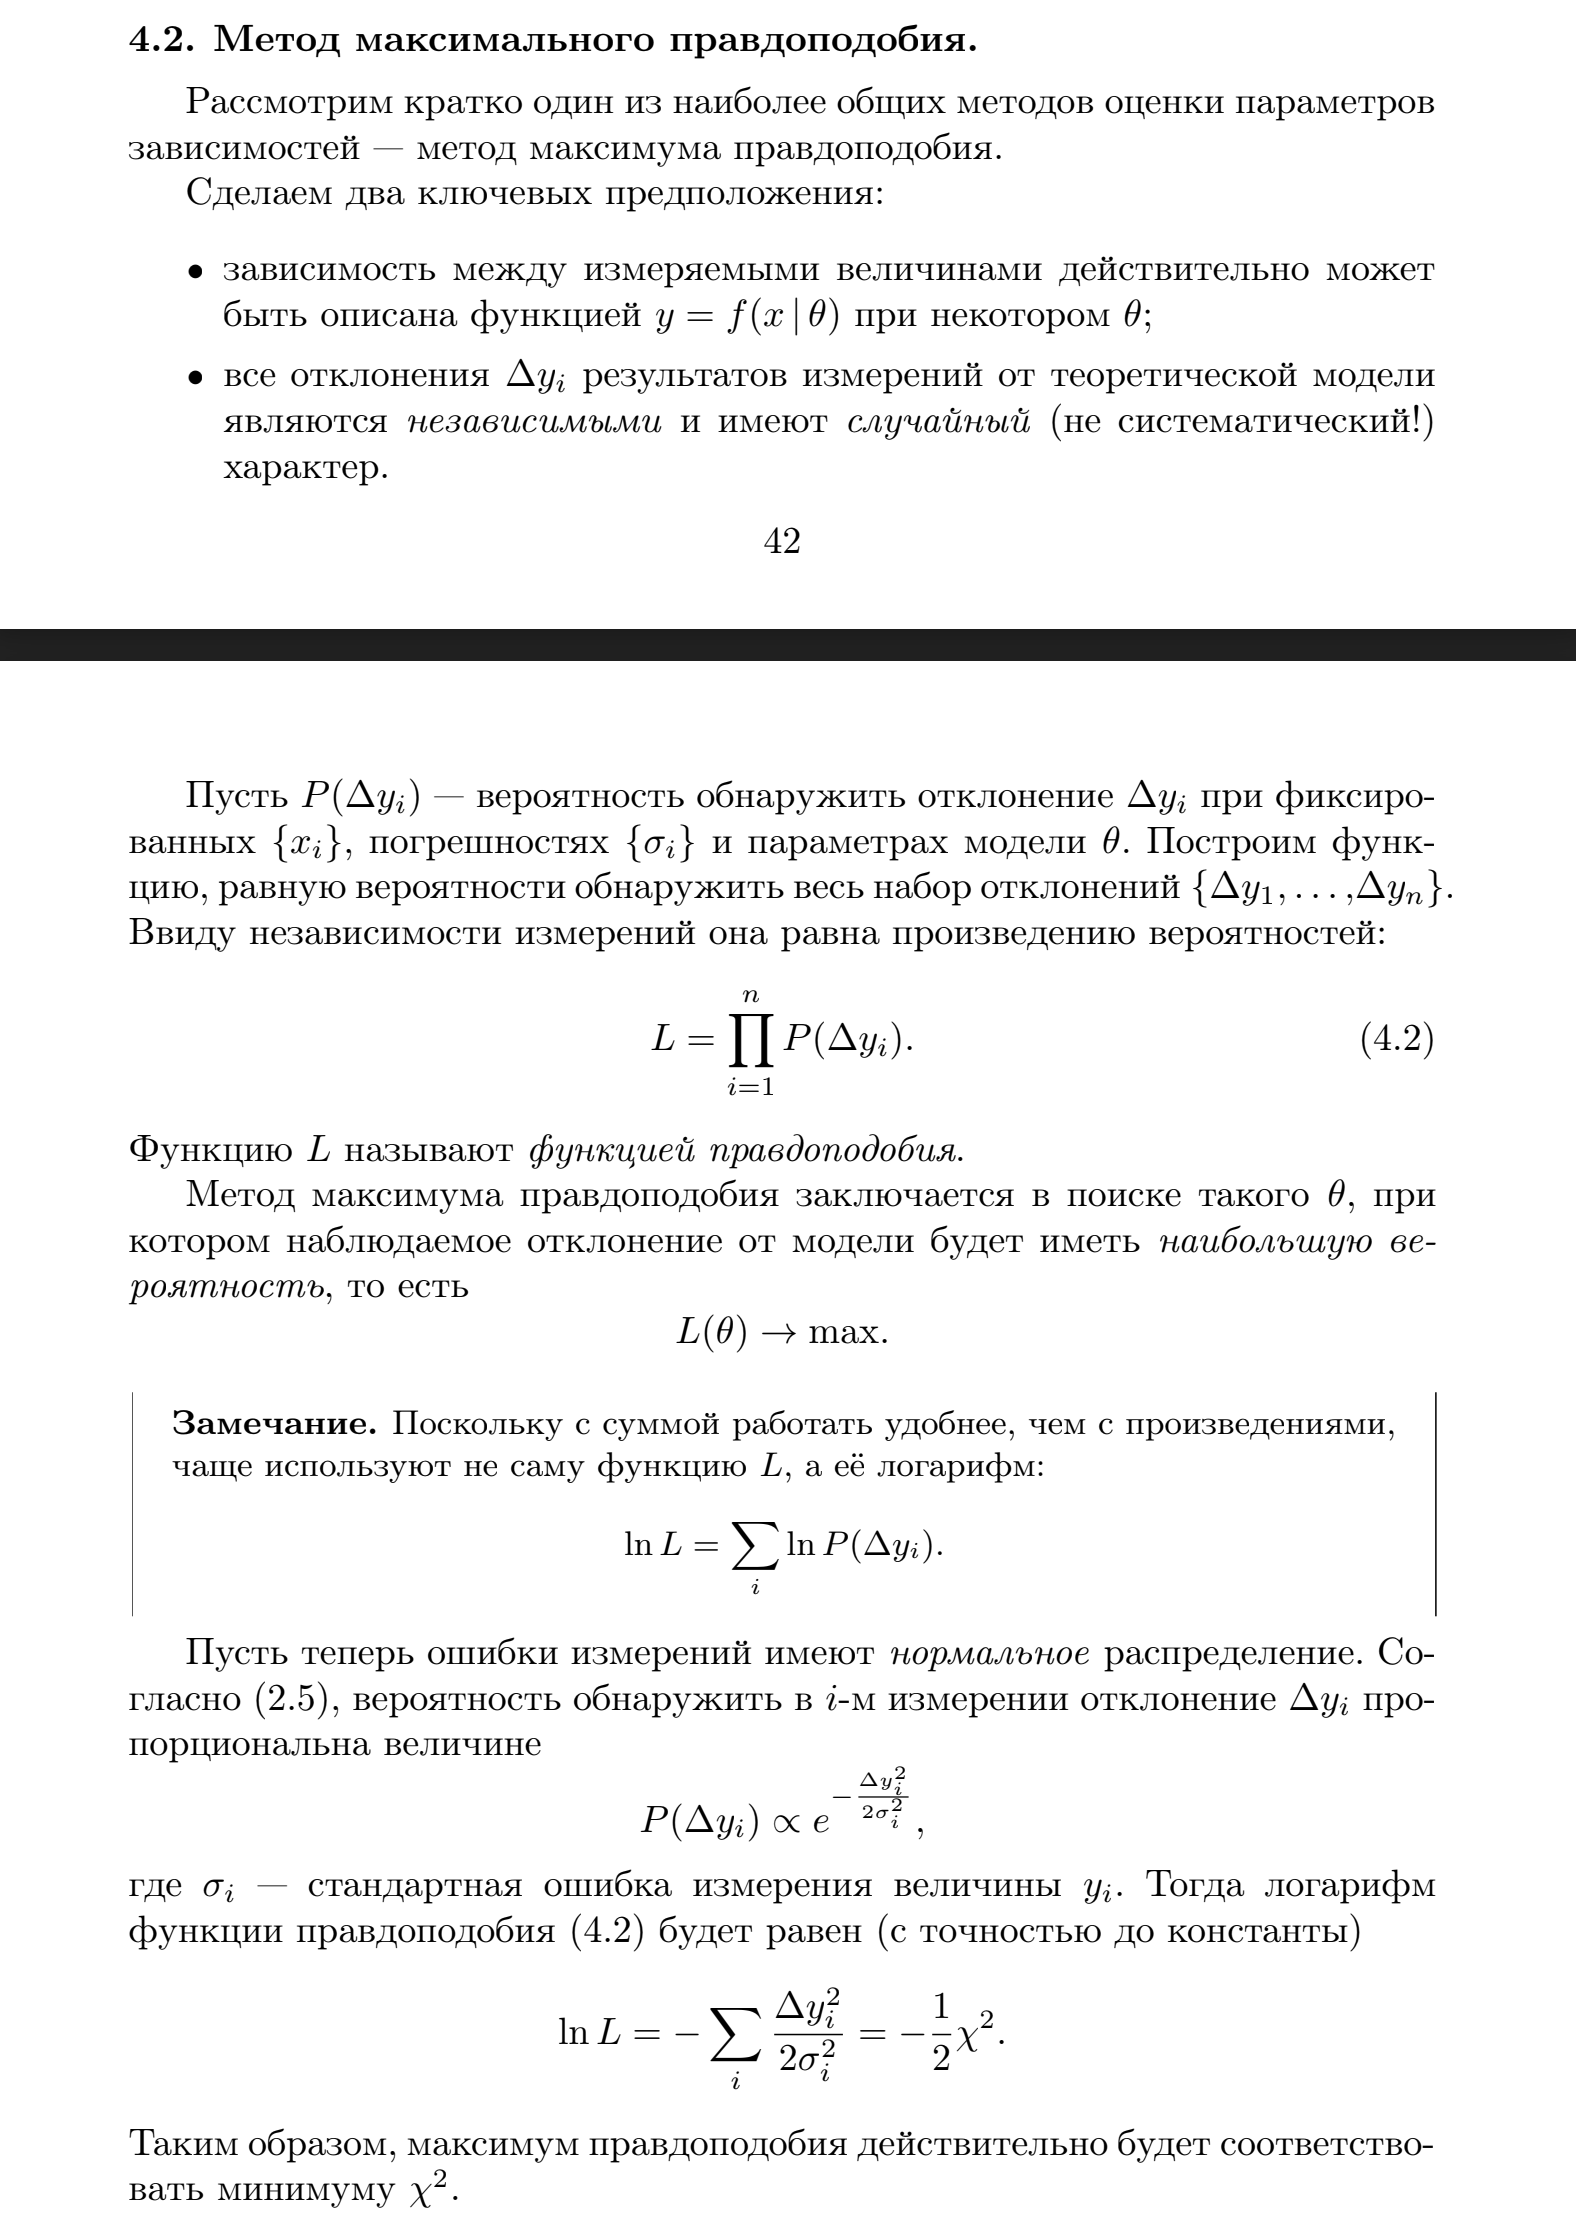
\includegraphics[width=0.8\paperwidth, center]{метод максимального правдоподобия}
Фрагмент отсюда \href{https://drive.google.com/file/d/11M5yI5y8wDZ0q8MtQzv-y28AN6DKgBDz/view}{П.В. Попов, А.А. Нозик \textit{Обработка результатов учебного эксперимента}}

\subsection{Погрешность функции}
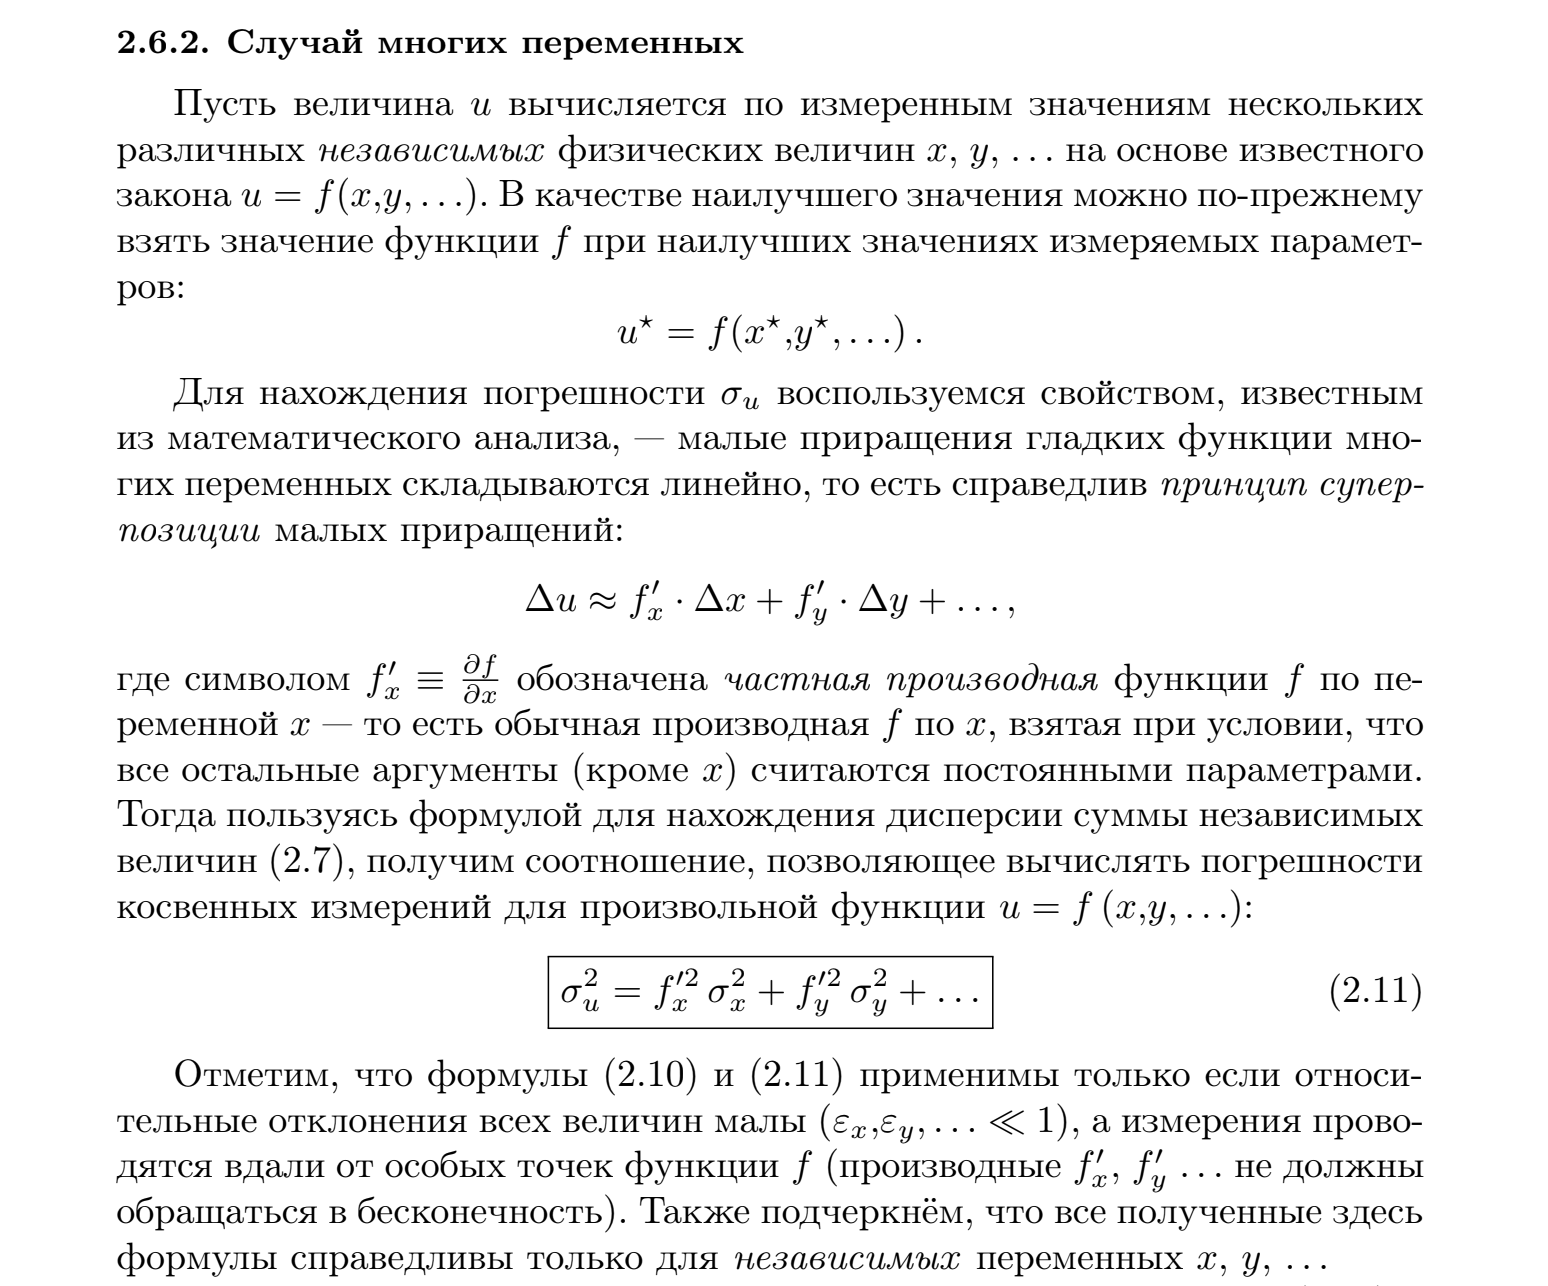
\includegraphics[width=0.8\paperwidth, center]{погрешность_функции.png}
Взято оттуда же.
Убедиться в том, на сколько этот вывод некорректный можно рассмотрев такой пример.

\[ f(x, y) = \frac{x}{y} \]
Имея измерение $t \pm \Delta t$, рассчитаем значение
\[ f(t, t) \equiv 1 \]
Понятно, что погрешность этого результата нулевая, а формула даст нам
ненулевую. Далее будет показано, как в случае зависимых переменных считать погрешность
функции, а при определении параметров методом аппроксимации они получаются зависимыми.
Также будет показано, как считаются погрешности параметров и их дисперсии.


\section{Основная часть}
\subsection{Дисперисия параметров аппроксимации}
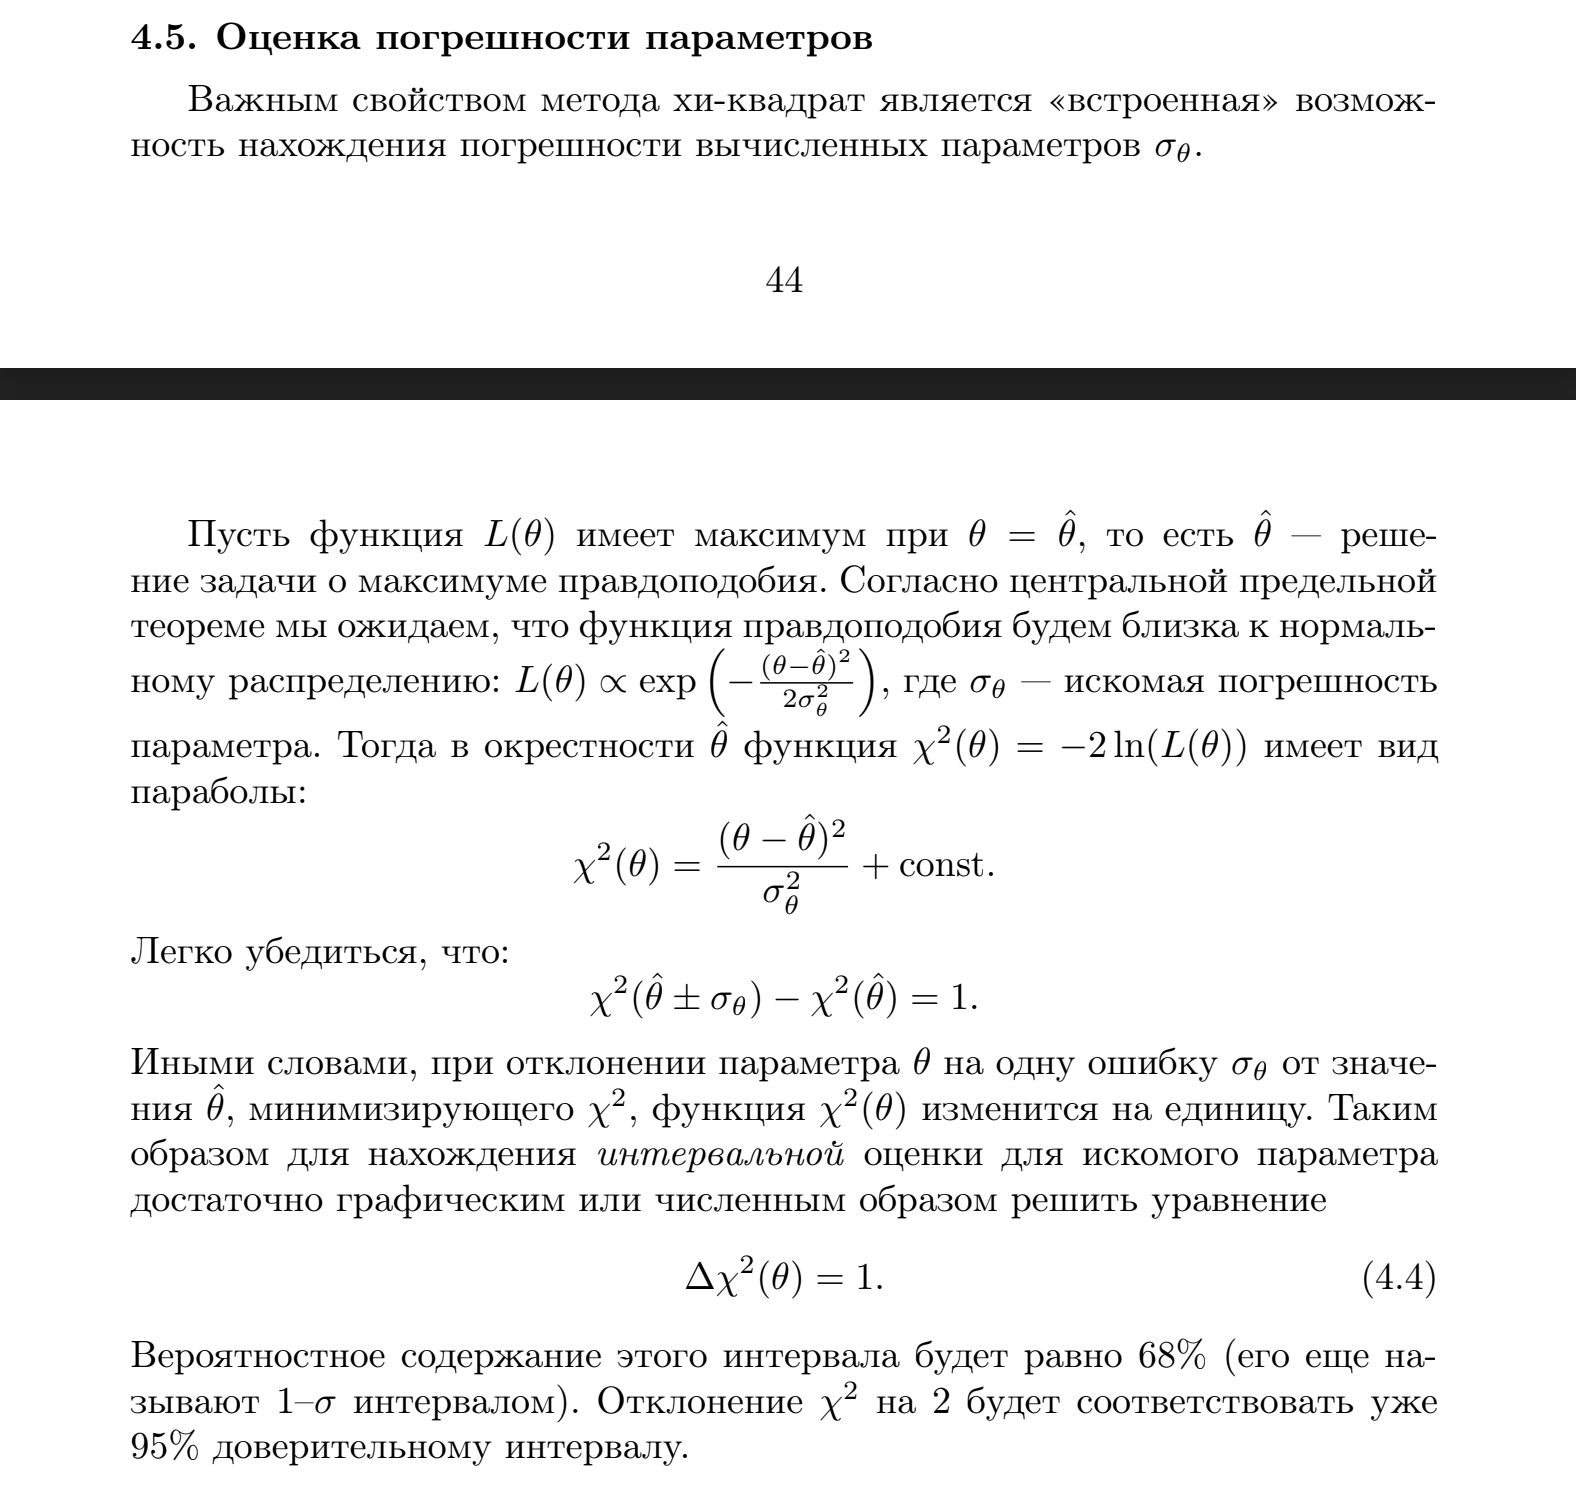
\includegraphics[width=0.8\paperwidth, center]{погрешность_параметров.png}

Отмечу также, что среднеквадратичное отклонение можно получить взяв вторую производную
\[ \frac{\partial^2 \chi^2(\theta)}{\partial \theta^2} = \frac{2}{\sigma_\theta^2}\]

Теперь рассмотрим случай нескольких переменных. По определению запишем
погрешность функции от нескольких переменных.

\[ \sigma_f^2 = M[\left(f(x+\Delta x, y + \Delta y) - f(x, y)\right)^2] 
\approx M[(\d{x}f\Delta x + \d{y}f\Delta y)^2]\]
\[ = M[(\d{x}f)^2\Delta x^2] + M[2\d{x}f\Delta x \d{y}f\Delta y] + M[(\d{y}f)^2\Delta y^2] \]
\[ = (\d{x}f)^2M[\Delta x^2] + 2\d{x}f \d{y}f M[\Delta x \Delta y] + (\d{y}f)^2 M[\Delta y^2] \]
\[ = (\d{x}f)^2\sigma_x^2 + 2\d{x}f \d{y}f M[\Delta x \Delta y] + (\d{y}f)^2 \sigma_y^2 \]
Остаётся множитель $M[\Delta x \Delta y]$, который не выражается через дисперсии $x$ и $y$. 
Он показывает связь между природой погрешности $x$ и $y$. Называется это ковариацией. В случае, если ошибки независимые,

\[ M[\Delta x \Delta y] = M[\Delta x] M[\Delta y] = 0\cdot0\]
Разберёмся как можно рассчитать ковариацию параметров аппроксимации.
\subsection{Рассчёт ковариации}

Разложим $\chi^2(\theta_i)$ функцию всех определяемых параметров вблизи минимума
как функцию от двух параметров ($\theta_1$ и $\theta_2$) по формуле Тейлор до первого неисчезающего порядка.
Будем считать, что значение параметров соответствующее минимуму равно нулю, чтобы не писать
лишний раз $\Delta$
Как было показано выше разложение будет иметь такой вид
\[ \chi^2(x, y) \approx const + \frac{\partial^2\chi^2(x, y)}{\partial x^2}\frac{\Delta x^2}{2} +
\frac{\partial^2\chi^2(x, y)}{\partial y^2}\frac{\Delta y^2}{2} + 
\frac{\partial\chi^2(x, y)}{\partial x}\frac{\partial \chi^2(x, y)}{\partial y}\Delta x \Delta y\]

Подставим выражение для второй производной через $\sigma$ и запишем множитель перекрёсного слагаемого через
обозначение 
\[corr = \frac{\frac{\partial\chi^2}{\partial x}\frac{\partial \chi^2}{\partial y}}{\sqrt{
    \frac{\partial^2\chi^2}{\partial x^2}\frac{\partial^2\chi^2}{\partial y^2}
}} =
-\frac{\d{\theta_1}\chi^2\d{\theta_2}\chi^2}{\sqrt{\d[2]{\theta_1}\chi^2\d[2]{\theta_2}\chi^2}} = \frac{D_{\theta_1\theta_2}}{\sigma_{\theta_1}\sigma_{\theta_2}}\]
($D_{\theta_1\theta_2} = -\frac{\d{\theta_1}\chi^2 \d{\theta_2}\chi 2}{2}$ тоже просто новое обозначение)
\[\chi^2-const =
\frac{\theta_1^2}{\sigma_{\theta_1}^2} - 2 \frac{corr \theta_1 \theta_2}{\sigma_{\theta_1} \sigma_{\theta_2}} + \frac{\theta_2^2}{\sigma_{\theta_2}^2}\]
Очень хочется сказать, что это квадрат суммы, но там перекрёстное слагаемое другое,
так что естественно будет сказать, что это скалярный квадрат суммы двух векторов.
Тогда угол между ними будет определять множитель этого перекрёстного слагаемого.
Чтобы было совсем красиво, возьмём эти базисные вектора не только не ортогональными, но и не нормированными.
Тогда
\[\left\lvert \vec{e}_{\theta_1} \right\rvert = \frac{1}{\sigma_{\theta_1}}\]
\[ \vec{\theta_1} = \theta_1\vec{e}_{\theta_1} \]
\[\left\lvert \vec{e}_{\theta_2} \right\rvert = \frac{1}{\sigma_{\theta_2}}\]
\[ \vec{\theta_2} = \theta_2\vec{e}_{\theta_2} \]
\[ \frac{corr}{\sigma_{\theta_1}\sigma_{\theta_2}} = -\vec{e}_{\theta_1}\vec{e}_{\theta_2} = \frac{-\cos(\alpha)}{\sigma_{\theta_1}\sigma_{\theta_2}}\]

\[ \frac{\theta_1^2}{\sigma_{\theta_1}^2} - 2 \frac{corr \theta_1 \theta_2}{\sigma_{\theta_1} \sigma_{\theta_2}} + \frac{\theta_2^2}{\sigma_{\theta_2}^2}
= \vec{\theta_1}^2 + 2\vec{\theta_1}\vec{\theta_2} + \vec{\theta_2}^2 =
(\vec{\theta_1} + \vec{\theta_2})^2 \]


Тогда в ортонормированном базисе($x$, $y$), где косинус угла между векторами $\vec{e}_{\theta_1}$ и $\vec{e}_{\theta_2}$ равен $corr$
выражение для $\chi^2$ равно просто скалярному квадрату вектора к точке, что есть квадрату
расстояния до начала координат. Тогда распределение вероятностей в этих координатах
равное $L = exp(-\frac{\chi^2}{2})$ сферически симметричное. Тогда можно посчитать среднее на
окружностях в таком пространстве и усреднить это по всем окружностям.
Найдём значения $\theta_1$ и $\theta_2$ как функцию новых координат.

\begin{figure}[H]
\centering
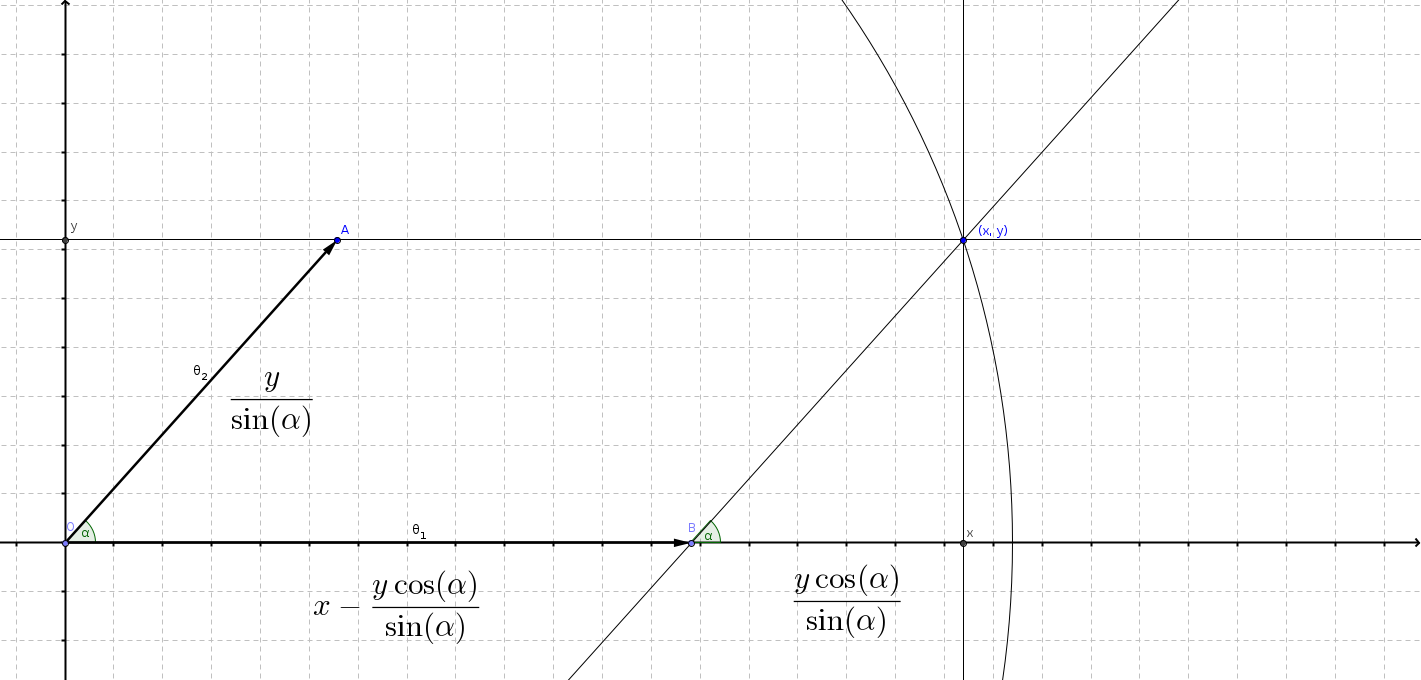
\includegraphics[width=1\textwidth]{geogebra_graph_3.png}
\caption{Рисунок в ортонормированном базисе $(x, y)$}
\label{fig:1}
\end{figure}

Возьмем точку $(x, y)$ и разложим ее по базису $\vec{e}_{\theta_1}$, $\vec{e}_{\theta_2}$ (см. рис. \ref{fig:1}).

Из простых геометрических соображений выражаем длины векторов $\vec{\theta_1}$ и $\vec{\theta_2}$ через
координаты и $\alpha$ - угол между единичными векторами.

\[ \left\lvert  \vec{\theta_2} \right\rvert = \left\lvert \vec{e}_{\theta_2} \right\rvert \theta_2 = \frac{y}{\sin(\alpha)} \]
\[ \left\lvert  \vec{\theta_1} \right\rvert = \left\lvert \vec{e}_{\theta_1} \right\rvert \theta_1 = x - \frac{y\cos(\alpha)}{\sin(\alpha)}
= x - \cos(\alpha)\left\lvert  \vec{\theta_2} \right\rvert \]

Теперь нужно усреднить по окружности выражение
\[ \langle \theta_1\theta_2\rangle =
\sigma_1\sigma_2 \langle \left\lvert  \vec{\theta_2} \right\rvert
\left\lvert  \vec{\theta_1} \right\rvert\rangle
= \sigma_1\sigma_2 \langle \left\lvert  \vec{\theta_2} \right\rvert
\left(  x - \cos(\alpha) \frac{\theta_2}{\sigma_2}  \right)\rangle
= \sigma_1\sigma_2 \left(
\frac{\langle xy\rangle}{\sin{\alpha}}  -
\cos(\alpha) \frac{\langle\theta_2^2\rangle }{\sigma_2^2}  \right) \]

Теперь нужно заметить, что среднее $\langle xy \rangle$ равно нулю. Это понятно например из того,
что при каждом $x$ распределение вероятности $y$ симметрично относительно нуля.
Среднее от произведения $\langle \theta_2^2\rangle$ при усреднении сначала по окружности, а потом
по всем таким окружностям будет тем же, чем и при усреднении по всему вероятностному пространству, то есть
просто среденеквадратичным отклонением (мы договорились, что у $\theta_2$ отклонение от среднего равно значению).
Тогда
\[ \langle \theta_1\theta_2\rangle = -\cos(\alpha)\sigma_1\sigma_2 \frac{\sigma_2^2}{\sigma_2^2} =
\sigma_1\sigma_2 corr = D_{\theta_1\theta_2} \]
В последних равенствах просто подставлены обозначения введенные выше по определению.
Таким образом мы выразили ковариацию двух параметров через коэффициенты разложения $\chi^2$ вблизи минимума

Далее $D_{xy} = \langle \Delta x \Delta y \rangle = \langle (x-\langle x\rangle)(y-\langle y\rangle) \rangle = \langle xy\rangle - \langle x\rangle \langle y \rangle$ будет использоваться как обозначение ковариации $x$ и $y$,
а дисперсию будем обозначать как ковариацию величины с самой собой $D_{xx} = \sigma_x^2$

Перепишем ковариацию через начальные частные производные
\[  D_{\theta_1\theta_2} = -\frac{\d{\theta_1}\chi^2 \d{\theta_2}\chi^2}{2} \]

То есть умея брать производную у $\chi^2$ сможем найти и ковариацию параметров аппроксимации. Можно также по
аналогии с методом нахождения среднеквадратичного отклонению по приравниванию увеличения $\chi^2$ относительно
минимума к 1 приравнять изменение $\chi^2(\theta_1, \theta_2))$ относительно минимума к 1 получить численное решение уравнения

\[1 =
\frac{\theta_1^2}{D_{11}} - 2 \frac{D_{12}\theta_1\theta_2}{D_{11} D_{22}} + \frac{\theta_2^2}{D_{22}}\]
Где символ $\theta$ в индексах опущен для большей наглядности. Решением будет эллипс, по параметрам которого при большом
желании тоже можно будет оценить параметры и получить ковариацию.

\section{Погрешность функции от зависимых переменных}

В случае зависимх переменных  слогаемые с ковариациями ($\langle \theta_1\theta_2\rangle$)
не будет нулевым. Распишем по определению погрешность через линейное приближение функции.
\[ \langle \Delta f(\theta)^2 \rangle = 
\langle (f(\theta + \Delta \theta)-f(\theta))^2\rangle
= \langle (\sum_{i=1}^{n} \Delta f(\Delta \theta_i))^2\rangle
= \langle \sum_{i=1}^{n}\sum_{j=1}^{n} \Delta f(\Delta \theta_i)\Delta f(\Delta \theta_j) \rangle =\]
\[= \sum_{i=1}^{n}\sum_{j=1}^{n} \langle\Delta\theta_i \Delta\theta_j \rangle \d{\theta_i} f \d{\theta_j} f 
= \sum_{i=1}^{n}\sum_{j=1}^{n} D_{\theta_i\theta_j} \d{\theta_i} f \d{\theta_j} f \]

 Где  сначала $\Delta \theta_i$ множество параметров, где i-ый элемент изменён, а остальные нет, а потом просто изменение i-ого аргумента,
  $\Delta f(\Delta \theta_i) = f(\Delta \theta_i) - f(\theta_i)$.

При обработке данных может быть удобнее использовать формулу через численную частную производную и корреляцию.
\[  \sum_{i=1}^{n}\sum_{j=1}^{n} corr_{ij}\Delta f(\Delta \theta_i)\Delta f(\Delta \theta_j) \]
Где уже $\Delta \theta_i$ множество параментов $\theta$ в котором i-ый параметр изменили на $\sigma_{\theta_i}$ 
\section{Вывод}
% напишу формулки, полезные на практике 

\end{document}